\documentclass{article}
\usepackage[utf8]{inputenc}
\usepackage[left=2cm, right=4cm, top=2cm]{geometry}
\usepackage{graphicx}
\graphicspath{ {../../../figures/snn/} }

\title{Convolutional Spiking Neural Networks}
\author{Daniel Saunders}

\begin{document}

\maketitle

This document tracks the progress of the BINDS lab on studying convolutional spiking neural networks (C-SNNs). No distinction is made between computational \textit{layers} and networks which use said layers; e.g., a \textit{convolutional SNN} is that which uses one or more \textit{convolutional layers}. \\

\textbf{Note}: All \texttt{code} is assumed to be Python + BindsNET syntax.

\section{Two layer locally connected SNNs}

An layer of \texttt{Input} neurons (layer \texttt{X}) equal to the size of the input data (e.g., MNIST or CIFAR-10) is connected via a \texttt{LocallyConnectedLayer} (\textbf{to be implemented}) with STDP-modifiable synapses to a layer of \texttt{AdaptiveLIFNodes} or \texttt{DiehlAndCook2015Nodes} (layer \texttt{Y}). Layer \texttt{Y} is recurrently connected to itself with inhibitory synapses via a \texttt{Connection}, the structure of which is a design choice (to be discussed in section \ref{ss:recurrent connectivity}).

\section{Two layer convolutional SNNs}

\subsection{Basic structure}

An layer of \texttt{Input} neurons (layer \texttt{X}) equal to the size of the input data (e.g., MNIST or CIFAR-10) is connected via a \texttt{Conv2dConnection} with STDP-modifiable synapses to a layer of \texttt{AdaptiveLIFNodes} or \texttt{DiehlAndCook2015Nodes} (layer \texttt{Y}). Layer \texttt{Y} is recurrently connected to itself with inhibitory synapses via a \texttt{Connection}.

Layer \texttt{Y} may be driven by \texttt{bernoulli()}- or \texttt{poisson()}-distributed spikes parametrized by the input data; since the networks are operating in an effectively rate-based regime, Bernoulli spikes may be preferred for efficiency reasons. \textbf{Note}: The implementation of \texttt{poisson()} may be slightly incorrect at this stage.

\begin{figure}[h]
	\centering
	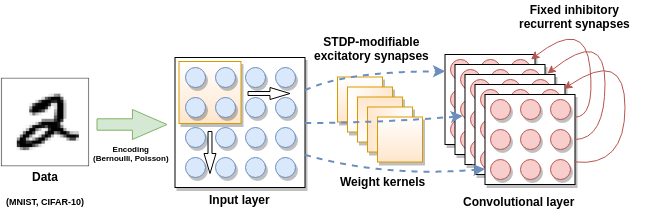
\includegraphics[width=0.8\textwidth]{two_layer_convolutional_snn.png}
	\caption{Schematic diagram of the structure of a two-layer convolutional spiking neural network. For ease of presentation, all data, layers, and weight kernels are depicted as two-dimensional (as in the case of gray-scale image processing). Input data encoded into spike trains is used for the activity of an input layer. Weight kernels are ``slid'' across the input space, multiplied by the input activations, and projected to unique neurons in the corresponding sub-population in the convolutional layer (one per weight kernel). The convolutional layer has inhibitory, recurrent connections, establishing a competition for spiking activity.}
\end{figure}

The goal of the convolutional layer is to learn a (compact) set of weight kernels (filters) which reliably detect salient features in the input space. The weight kernels ``slide'' across the input space with a regular horizontal and vertical \textit{stride}, and are multiplied by the activations at each input location to produce an activation value for a unique neuron in the next layer.

This technique has been successful in convolutional neural networks (CNNs) of deep learning; however, the neural model is much simplified, and the network can be efficiently trained using optimization techniques (stochastic gradient descent (SGD)). In the case of SNNs, the input activations are converted into spike trains, and the output of the convolution can be interpreted as current to be injected into the post-synaptic layer.

\section{Modifications}

This section describes some algorithmic and architectural modifications to the above described networks. Some changes apply to all network structures; when possible, it will be noted when changes apply to certain structures and not others.

\subsection{Recurrent connectivity}
\label{ss:recurrent connectivity}

There are some variants of connectivity of the recurrent connection for layer \texttt{Y}.

\subsubsection{Inhibit all other neurons}

In the spirit of Diehl \& Cook 2015, each neuron in layer \texttt{Y} is connected with an inhibitory synapse to all other neurons in the layer. This creates a simple competitive mechanism: when a neuron fires, all other neurons are damped, allowing the ``winning'' neuron to continue firing and to update its weights in the direction of the current input pattern. This is similar to the idea of a \textit{winner-take-all (WTA) circuit}.

The result of this training is improved clarity of weight kernels. Since (typically) only one neuron is able to fire consistently, that neuron can significantly update the weights of the filter (using STDP) in the direction of the stimulus that is firing it; i.e., the input data.

\subsubsection{Inhibit all neurons with same spatial field}

This change applies only to the \textit{locally connected networks}.

Only neurons in layer \texttt{Y} which receive connections from the same neurons of the input layer are recurrently connected with inhibitory synapses. The result of this change is that only neurons with the same \textit{spatial field} are involved in a miniature competition akin to that of the Diehl and Cook 2015 network. Each spatial field \textit{sub-population} is involved in the WTA-like circuit, and thus, at most one neuron from each sub-population can be the ``winner'' of the spiking competition per input example.

\subsection{Architectural modifications}

\subsubsection{Duplicate layer \texttt{Y} without recurrent connectivity}

In the typical setup, the convolutional layer \texttt{Y} has recurrent inhibitory connections that cause competition to take place between neurons, thereby allowing ``winning'' neurons to change their weights in the direction of the stimulus firing them. However, this connectivity also causes sparse activation in the layer, implying that it may be difficult to use the layer's output as input to downstream network layers (depending on the degree of sparseness).

To remedy this issue, we may \textit{duplicate} the layer \texttt{Y}, creating \texttt{Y'}, which receives connections from the input layer \texttt{X} with weights tied to those of the layer {Y}. The activation of layer \texttt{Y'} does not effect the modification of these connection weights, and there are no recurrent inhibitory connections in the layer. This allows \texttt{Y'} to activate much more than \texttt{Y}, and its output may therefore be more useful as input to downstream network components.

\end{document}
